\documentclass[nobib]{tufte-handout}

%\\geometry{showframe}% for debugging purposes -- displays the margins

\newcommand{\bra}[1]{\left(#1\right)}
\usepackage{clrscode3e}
\usepackage{hyperref}
\usepackage[activate={true,nocompatibility},final,tracking=true,kerning=true,spacing=true,factor=1100,stretch=10,shrink=10]{microtype}
\usepackage{color}

% Fixes captions and images being cut off
\usepackage{marginfix}

\usepackage{tikz}
\usepackage{amsmath,amsthm}
\usetikzlibrary{shapes}
\usetikzlibrary{positioning}

% Set up the images/graphics package
\usepackage{graphicx}
\setkeys{Gin}{width=\linewidth,totalheight=\textheight,keepaspectratio}
\graphicspath{{.}}

\title{Notes for PHYS 27200 - Electric And Magnetic Interactions}
\author[Ezekiel Ulrich]{Ezekiel Ulrich}
\date{\today}  % if the \date{} command is left out, the current date will be used

% The following package makes prettier tables.  We're all about the bling!
\usepackage{booktabs}

% The units package provides nice, non-stacked fractions and better spacing
% for units.
\usepackage{units}

% The fancyvrb package lets us customize the formatting of verbatim
% environments.  We use a slightly smaller font.
\usepackage{fancyvrb}
\fvset{fontsize=\normalsize}

% Small sections of multiple columns
\usepackage{multicol}

% These commands are used to pretty-print LaTeX commands
\newcommand{\doccmd}[1]{\texttt{\textbackslash#1}}% command name -- adds backslash automatically
\newcommand{\docopt}[1]{\ensuremath{\langle}\textrm{\textit{#1}}\ensuremath{\rangle}}% optional command argument
\newcommand{\docarg}[1]{\textrm{\textit{#1}}}% (required) command argument
\newenvironment{docspec}{\begin{quote}\noindent}{\end{quote}}% command specification environment
\newcommand{\docenv}[1]{\textsf{#1}}% environment name
\newcommand{\docpkg}[1]{\texttt{#1}}% package name
\newcommand{\doccls}[1]{\texttt{#1}}% document class name
\newcommand{\docclsopt}[1]{\texttt{#1}}% document class option name

% Define a custom command for definitions
\newcommand{\defn}[2]{\noindent\textbf{#1}:\ #2}

\begin{document}

\maketitle

\begin{abstract}
These are lecture notes for fall 2023 PHYS 27200 at Purdue. Modify, use, and distribute as you please.
\end{abstract}

\tableofcontents

\section{Course Introduction}

This is a calculus-based physics course using concepts of electric and magnetic fields and an atomic description of
matter to describe polarization, fields produced by charge distributions, potential, electrical circuits,
magnetic forces, induction, and related topics, leading to Maxwell's equations and electromagnetic
radiation and an introduction to waves and interference. 3-D graphical simulations and numerical problem
solving by computer are employed throughout. For more information, consult the syllabus.

\section{Equations}

\begin{enumerate}
    \item Coulomb's Law: $\vec{F} = \frac{1}{4\pi \epsilon_0}\frac{q_1 q_2}{r^2}\hat{r}$
    \item Electric field due to a point or charged sphere: $\vec{E_1} = \frac{1}{4\pi \epsilon_0}\frac{q_1}{r^2}\hat{r}$
    \item Force due to electric field: $\vec{F_2} = E_1 q_2$
    \item Dipole moment between charges $-q$ and $q$ separated by $\vec{s}$: $\vec{p} = q\vec{s}$
    \item Electric field on dipole axis: $\vec{E} = \frac{1}{4\pi \epsilon_0}\frac{2sq}{r^3}\hat{p}$
    \item Electric field on dipole bisecting plane: $\vec{E} = \frac{-1}{4 \pi \epsilon_0}\frac{sq}{r^3}\hat{p}$
\end{enumerate}

\pagebreak

\section{Electric charge}

\defn{Electric Charge}{Electric charge is an intrinsic characteristic of the
fundamental particles that make up objects.}

\marginnote{It was mentioned in class that mass is likewise intrinsic. 
However, when discussing the Higgs field's role in giving particles mass, 
the distinction between mass as an intrinsic or emergent property becomes 
more nuanced. The mass of elementary particles like electrons and quarks is 
emergent in the sense that it arises from their interaction with the Higgs 
field, which itself is a fundamental aspect of the universe.}

\defn{Conservation of charge}{The net charge of a \emph{closed system} never changes}

Objects can have negative, zero, or postive charge. 
Charges are always multiples of the \emph{elementary charge} $e = 1.60217662(63) \times 10^{-19} C$

\defn{Coulomb (C)}{One coulomb is the amount of charge that is
transferred through the cross section of a wire in 1 second
when there is a current of 1 ampere in the wire.}

The charges of elementary particles are listed below.
\begin{table}[ht]
    \centering
    \begin{tabular}{@{}ll@{}}
    \toprule
    Particle & Charge (elementary charge, $e$) \\
    \midrule
    Electron ($e^-$) & $-1$ \\
    Positron ($e^+$) & $+1$ \\
    Proton ($p^+$) & $+1$ \\
    Anti-proton ($p^-$) & $-1$ \\
    Neutron& $0$ \\
    Anti-neutron & $0$ \\
    Photon& $0$ \\
    \bottomrule
    \end{tabular}
    \end{table}

\defn{Point Charge}{A charged object whose
radius is much smaller than the distance
between itself and all other objects of
interest.}

The magnitude of electric force between two point charges is d
irectly proportional to the magnitude of each charge and 
inversely proportional to the distance squared. Specifically:
\[F = \frac{1}{4\pi \epsilon_0}\frac{q_1 q_2}{r^2}\]
This is Coulomb's Law. Note the direction of the force changes
with the sign of the charges involved. Like repels like and opposites
attract. 

\section{Electric field}

\begin{marginfigure}
    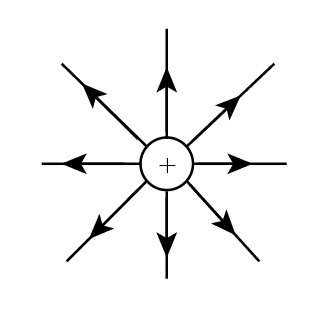
\includegraphics{images/electricfieldlines.jpg}
    \caption{An eletric field coming from point charge. 
    Notice how the densities of the lines vary with distance from the source.}
    \label{fig:electric-field-lines-point-charge}
\end{marginfigure}
Consider a charged particle. We can represent its effect
by drawing vectors that show the path a positively charged 
particle would follow if placed within its influence. These lines represent the 
electric field of the charged particle. The greater the density of the lines, the greater 
the strength of the electric field. Note that at the origin, the force is
undefined (infinite), since $|r| = 0$. 

There are many types of fields, which can be either scalar 
or vector. 
\marginnote{Technically, fields can be the more general tensor,
or even the fascinating and exotic spinor!}
For example, a temperature map is a scalar field, since
each point is associated with a scalar (the temperature at that 
point). A map of fluid velocity is a vector field, since each point 
is associated with a vector (the velocity of the fluid at that point).
For a particle, the eletric field vector at any point is given by
\[\vec{E_1} = \frac{1}{4\pi \epsilon_0}\frac{q_1}{r^2}\hat{r}\]
The direction in which the field lines point depends on the 
sign of the charge. If the charge is negative, the field lines point in.
If it is positive, the field lines point out. A useful mnemonic is
to think of the charge as someone's STD test results. If it's negative,
others will go for them and the lines point in. If it's positive, everyone
will try to get away and the lines point out.

Consider the relative strengths of the electric and 
gravitational fields. The gravitational force is given by
$F_g = G\frac{m_1m_2}{r^2}\hat{r}$, with $m_{electron} = 9 \times 10^{-31} kg$
and $m_{proton} = 1.7 \times 10^{-27} kg$. If we consider a hydrogen atom,  
then $r = 5.3 \times 10^{-11} m$. With $G = 6.7 \times 10^{-11}$, we have 
\[F_g = \frac{(1.7 \times 10^{-27})(9 \times 10^{-31})(6.7 \times 10^{-11})}{(5.3 \times 10^{-11})^2} \approx O(10^{-46})N\]
Now, the eletric force is given by $\vec{F} = \frac{1}{4\pi \epsilon_0}\frac{q_1 q_2}{r^2}\hat{r}$. 
The charge of a proton and eletric are $q_1 \approx q_2 \approx 1.6 \times 10^{-19} C$.
Ergo, since $\frac{1}{4\pi \epsilon_0} \approx 8.99 \times 10^9 \frac{Nm^2}{C^2}$, 
\[F_e = \frac{(8.99 \times 10^9 \frac{Nm^2}{C^2})(1.60\times10^{-19}C)^2}{(5.3\times10^{-11}m)^2} \approx O(10^-17)N\]
This means that $\frac{F_e}{F_g}\approx 2.27 \times 10^{39}$, meaning the eletric force is
much stronger for these masses and charges than gravity. On scales as large as humans and planets,
gravity is the dominant force because gravity is strictly additive.

For sufficient distances, the eletric field
of a uniformly charged spherical shell resembles
the eletric field of a point charge. 

\begin{marginfigure}
    \begin{center}
    \begin{tikzpicture}
        % Dot
        \fill (0,0) circle (1pt);
        % Arrow
        \draw[->] (0,0) -- (0,3);
    \end{tikzpicture}
    \end{center}

    \caption{Notice how a circle resembles a point from a great distance.}
    \label{fig:long-distance-point-sphere}
\end{marginfigure}

That means for $r>>R$, $\vec{E_{sphere}} = \frac{1}{4\pi \epsilon_0}\frac{q_1}{r^2}\hat{r}$
This holds only for outside the sphere. Inside, it can be shown that the electric field is zero. 

\defn{Superposition Principle}{The net electric field at a location in space is a
vector sum of the individual electric fields contributed by all
charged particles located elsewhere.}

To introduce systems with multiple sources of electric field lines, consider
the particle pair known as a dipole. Dipoles consist of one negatively charged
and one positively charged particle, like so:
\begin{marginfigure}
    \centering
    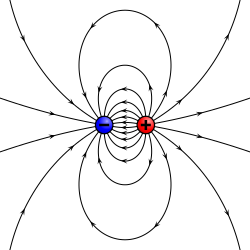
\includegraphics[width=\textwidth / 2]{images/VFPt_dipole_electric.svg.png}
    \caption{Two oppositely charged particles distanced from one another}
    \label{fig:dipole}
\end{marginfigure}

\defn{Dipole Moment}{The dipole moment is a way of expressing asymmetrical charge distribution.
It is a vector quantity, i.e. it has magnitude as well as definite directions.} The
dipole moment is given by the expression $\vec{p} = q\vec{d}$, where $q$ is
the charge on one end of the dipole and $\vec{d}$ is the distance between dipoles.

On the axis of the dipole (i.e. the lines
formed by the two particles), the electric field is 
\[\vec{E} = \frac{1}{4\pi \epsilon_0}\frac{2sq}{r^3}\hat{p}\]
On the bisecting plane (i.e., the plane exactly halfway from each 
point) the field is given by
\[\vec{E} = \frac{-1}{4 \pi \epsilon_0}\frac{sq}{r^3}\hat{p}\]
Where $r$ is the distance from the point to either dipole.
The force on a positive point charge $q_1$ a 
distance of $d$ away from the dipole, aligned with the dipole, and 
on the side of the negative charge is given by 
\[\vec{F}=q_1\vec{E_{dipole}}=q_1(\frac{-1}{4\pi \epsilon_0}\frac{2qs}{d^3},0,0)\]
Note that the field will be parallel to the axis of the dipole: this 
can simplfy vector calculations.
Now consider a dipole in a uniform electric field, like so:
\begin{figure}
    \caption{Dipole in uniform electric field}
    \center
    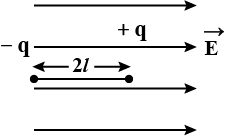
\includegraphics[width=\textwidth /2]{images/dipoleinuniformelectricfield.png}
\end{figure}
The positive end will be pulled to the right and the negative 
end to the left, exerting a torque given by $\vec{\tau} = \vec{p} \times \vec{E_{uniform}}$.
Note that by the definition of $\times$, $\tau = p E_{uniform} \sin{\theta}$, where $\theta$ is the
dipole's angle from horizontal. It can be shown that the potential
energy of a dipole in a uniform eletric field is $U = -\vec{p} \cdot \vec{E_{uniform}}$
and similarly as before (but now with $\cdot$) $U = -p E_{uniform} \cos{\theta}$. 
\end{document}
